\section{Preliminary Results}\label{section:results}

As a criteria of the project is to benchmark the performance of different frameworks against the performance of ROOT based HistFactory benchmarking of the different backends was carried out.
As a preliminary benchmark of the frameworks a one point CLs test was performed, in which XXXXX.
The results are shown against each other in Figure~\ref{fig:benchmark_backends}.
As a pure MXNet optimizer has not been implemented in pyhf at this time it has not yet been benchmarked, and so only backends that do have language specific optimizers have been compared to ROOT based HistFactory.

The preliminary results show that the computational backends that support automatic differentiation and built in parallelism show promising scaling behavior as the nature of the statistical fits becomes more computational difficult.
The optimizer for the NumPy pyhf backend is based on optimizers in SciPy, and while the NumPy backend optimizer does not currently have auto grad support it does show very good timing for lower computational difficulty problems.
Given that pyhf allows for fluidity in the choice of backend, this demonstrates a possible use case for automatically switching from the low overhead NumPy backend to a computational graph based backend as computational difficulty rises.

\begin{figure}
 \centering
 % Switch this out so can see the uncertainties
 % 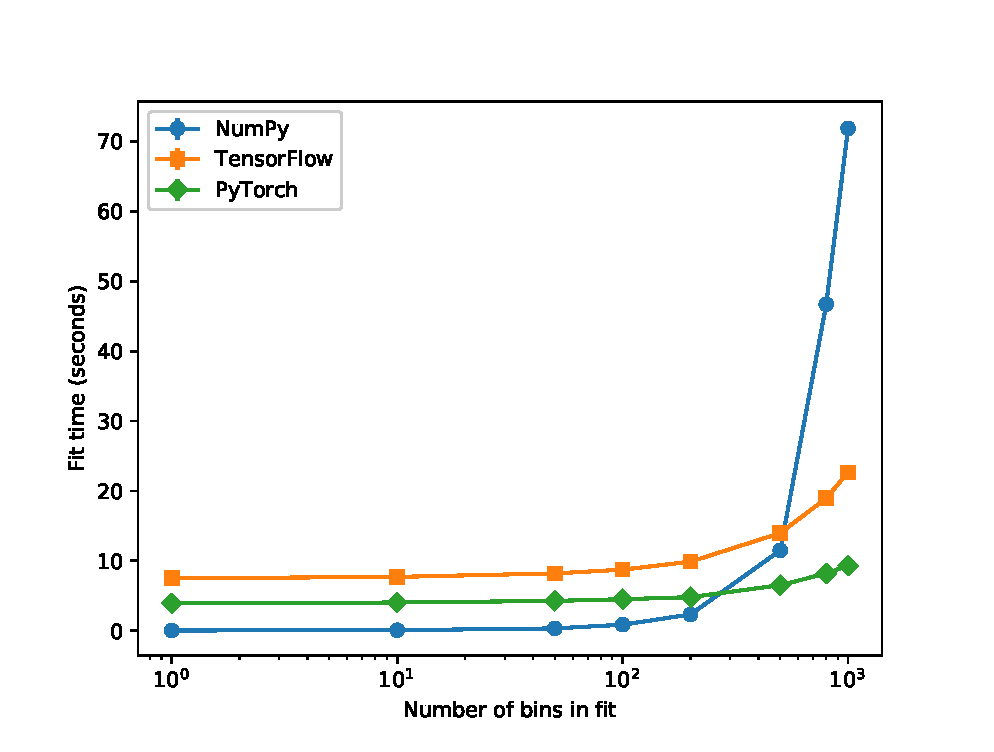
\includegraphics[width=0.9\linewidth]{benchmark_times.eps}
 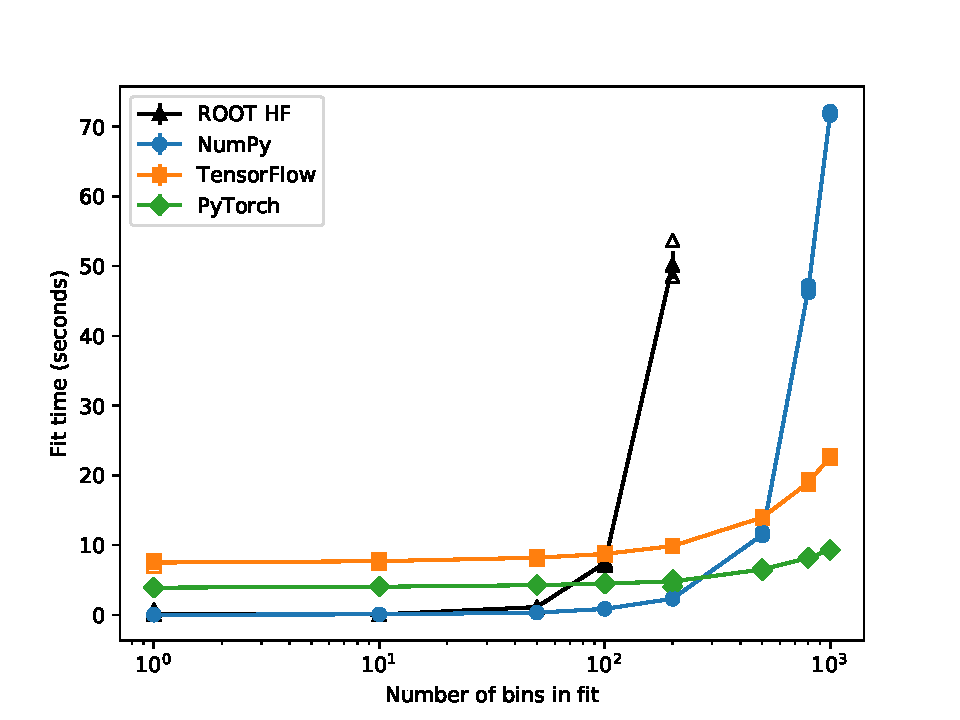
\includegraphics[width=0.8\linewidth]{benchmark_times.pdf}
 \caption{Comparison of the mean time needed to complete a one point CLs test for ROOT HistFactory and the NumPy, TensorFlow, and PyTorch pyhf backends vs. the number of bins in the associated fit.
  The model used is a simple one in which every bin has the same content to ensure that the fit will complete.
  In lieu of model complexity large numbers of bins are given to simulate difficult conditions for the fit.
  The binning choices used are $n_{\text{bins}} \in \left\{1, 10, 50, 100, 200, 500, 800, 1000\right\}$.
  For each binning choice the fit is repeated 5 times.
  For ROOT HistFactory only binning choices up to 200 are used as runtime became too long afterwards.
  The minimum and maximum time for each run are shown as open shapes corresponding to the shapes of the markers for each backend, and an uncertainty bar corresponding to 1 standard deviation is drawn (though it may be obscured by the markers).
 }\label{fig:benchmark_backends}
\end{figure}

\begin{figure}[htbp]
 \centering
 \subfigure[ROOT HistFactory]{%
  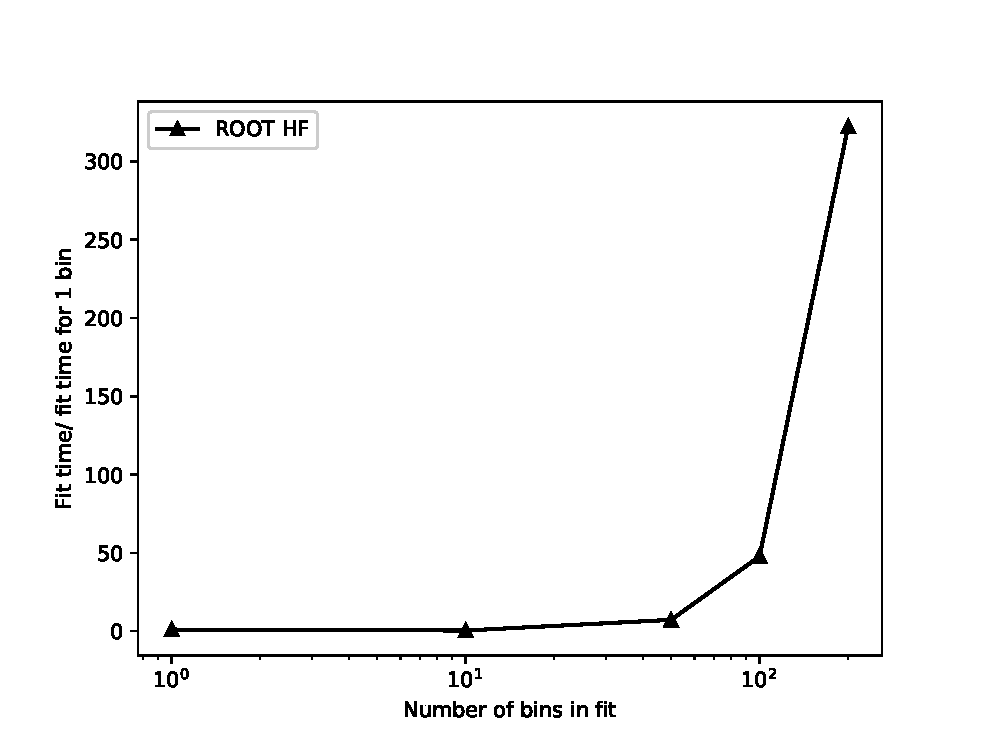
\includegraphics[width=0.5\textwidth]{relative_times_root_log.eps}\label{fig:relative_time_root_HF}%
 }\hfil
 \subfigure[NumPy backend]{%
  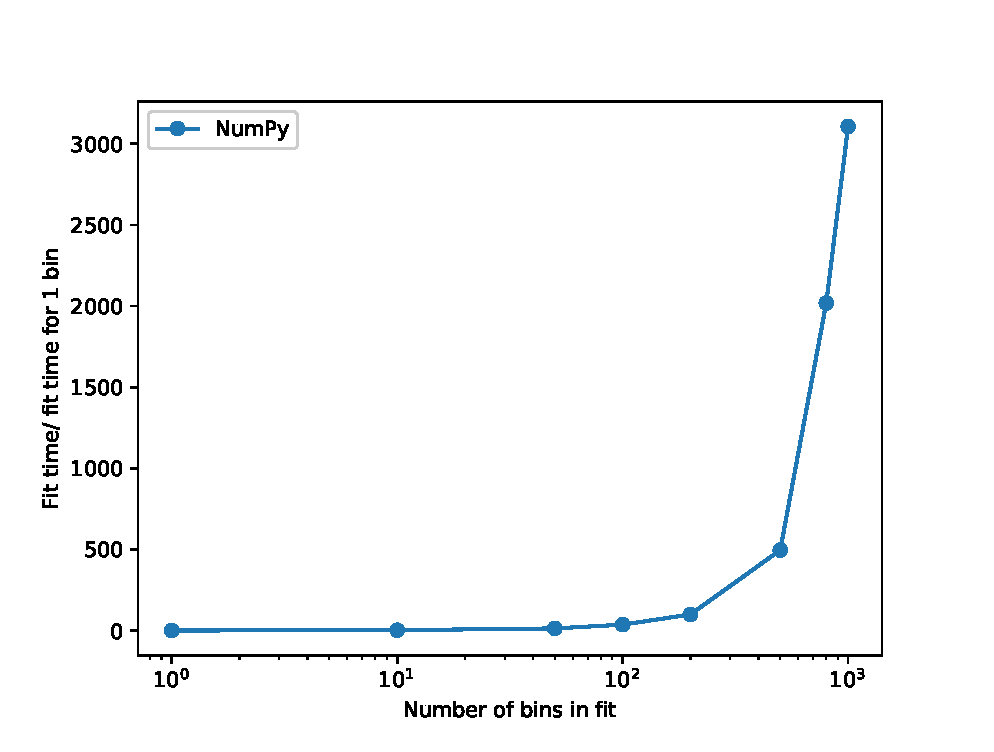
\includegraphics[width=0.5\textwidth]{relative_times_numpy_log.eps}\label{fig:relative_time_numpy}%
 }
 \subfigure[TensorFlow backend]{%
  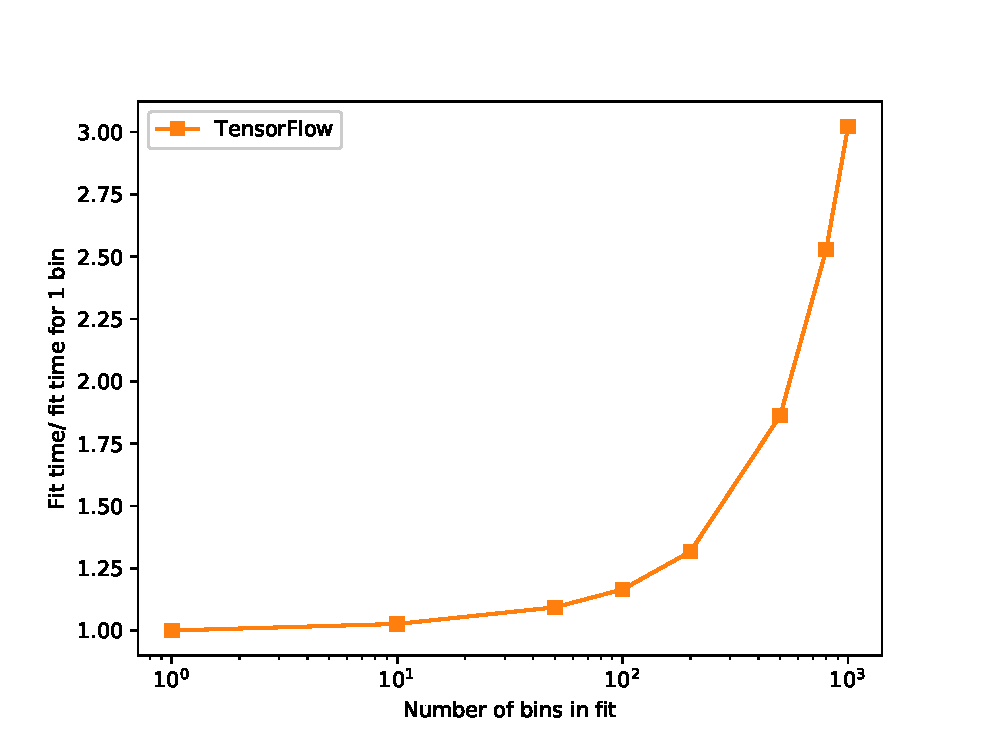
\includegraphics[width=0.5\textwidth]{relative_times_tensorflow_log.eps}\label{fig:relative_time_tensorflow}%
 }\hfil
 \subfigure[PyTorch backend]{%
  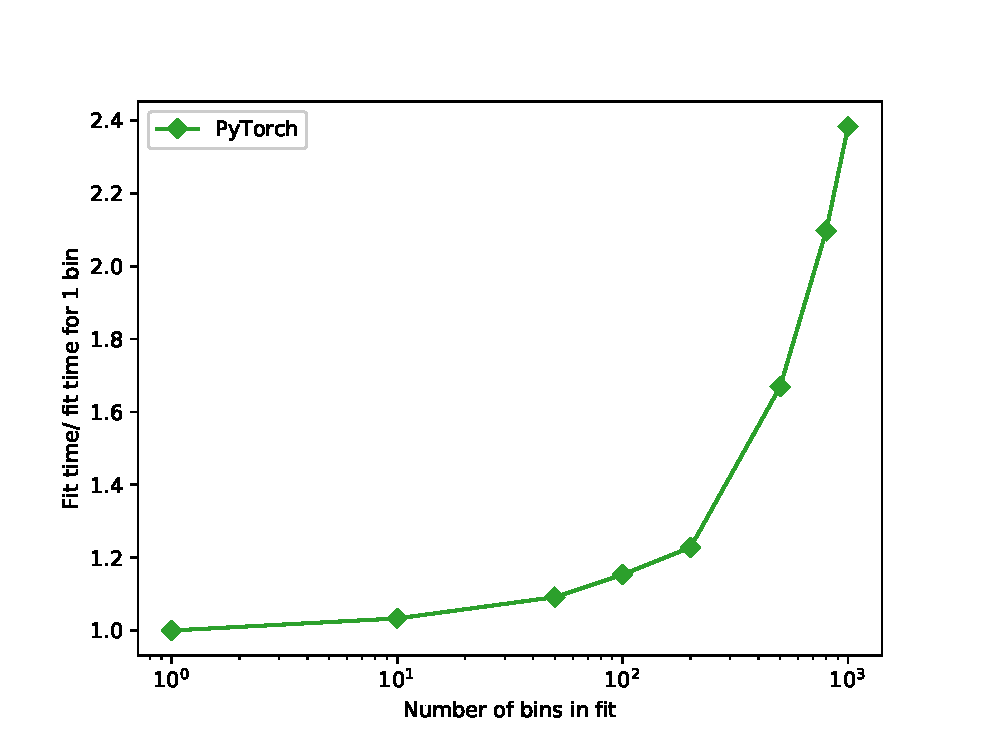
\includegraphics[width=0.5\textwidth]{relative_times_pytorch_log.eps}\label{fig:relative_time_pytorch}%
 }
 \caption{Comparison of the mean time needed to complete a one point CLs test for ROOT HistFactory and the pyhf backends for a number of bins in the associated fit relative to the time for a single bin.
  The model used is a simple one in which every bin has the same content to ensure that the fit will complete.
  The binning choices used are $n_{\text{bins}} \in \left\{1, 10, 50, 100, 200, 500, 800, 1000\right\}$.
  For ROOT HistFactory only binning choices up to 200 are used as runtime became too long afterwards.
 }
\end{figure}
